\documentclass[10pt,conference]{IEEEtran}

\usepackage{cite}
\usepackage{graphicx}
\DeclareGraphicsRule{.jfif}{jpg}{.jfif}{}
\usepackage{amsmath,amssymb,amsfonts}
\usepackage{algorithmic}
\usepackage{algorithm}
\usepackage{url}
\usepackage{hyperref}
\usepackage{booktabs}
\usepackage{array}
\usepackage{multirow}
\usepackage{microtype}

\hypersetup{
  colorlinks=true,
  linkcolor=blue,
  filecolor=magenta,
  urlcolor=cyan,
  citecolor=blue
}

\title{Cybersecurity Assurance of AI-Generated Scientific Claims in Autonomous Deep-Space Multi-Agent Systems}

\author{
  \IEEEauthorblockN{Abba Abdullahi Wakili}
  \IEEEauthorblockA{
    \textit{Independent Researcher}\\
    Kano, Nigeria\\
    \textit{B.Sc. Computer Science, Bayero University Kano (2025)}\\
    \href{mailto:abbaabdullahiwakeel@gmail.com}
    {abbaabdullahiwakeel@gmail.com}
  }
}

\begin{document}

\maketitle

\begin{abstract}
Autonomous deep-space missions must increasingly generate and evaluate scientific information with limited or delayed human oversight. This creates a cybersecurity assurance problem: how can mission operators assess the integrity and evidential trustworthiness of scientific claims produced by autonomous agents when communication delays, intermittent connectivity, sensor faults, and compromised probes prevent immediate human verification? Existing work provides important but separate building blocks, including spacecraft autonomy verification and validation, trusted-AI frameworks, multi-agent trust and reputation, provenance, secure delay-tolerant networking, and claim-level auditability for AI-generated research. This paper proposes TRUSTPASS, a layered architecture that combines evidence packages, sensor-health assessment, uncertainty, provenance and integrity metadata, cross-relay verification, and dynamic reputation. We formalize evidence aggregation and trust decisions, define a machine-verifiable Trust Passport schema, and model threats including compromised probes, false consensus, relay tampering, replay, provenance manipulation, and compromised reasoning components. We evaluate the architecture in a synthetic multi-agent simulation using 80 Monte Carlo trials per configuration. The revised evaluation includes component ablations, compromised-agent sweeps, and packet-loss experiments. Sensor-health and provenance/integrity weighting provide the largest gains under the tested configuration, while dynamic reputation is most useful for smaller constellations. Cross-relay verification and uncertainty weighting do not improve accuracy in every tested regime, exposing calibration and consensus-reinforcement limitations. The results constitute a controlled proof of concept, not a mission-ready validation.
\end{abstract}

\begin{IEEEkeywords}
autonomous spacecraft, deep-space systems, multi-agent systems, cybersecurity assurance, trust and reputation, provenance, uncertainty, AI-generated scientific claims, sensor fusion
\end{IEEEkeywords}

\section{Introduction}
\label{sec:introduction}

Deep-space missions face long communication delays, intermittent connectivity, constrained computation, and harsh operating environments. These conditions limit direct human control and motivate onboard autonomy for navigation, operations, observation planning, and scientific inference~\cite{cardoso2021review,feather2023assurance,nesnas2021autonomy}. As mission concepts become more ambitious, autonomous systems must make decisions when communication with Earth is slow or unavailable.

The increasing use of AI in space introduces an additional assurance challenge. An autonomous system may not only control a spacecraft but also interpret sensor data, prioritize observations, generate hypotheses, and produce scientific claims. Examples include claims such as ``water detected at location $X$,'' ``mineral composition $Y$ inferred,'' or ``anomaly $Z$ observed.'' A claim can be syntactically valid and cryptographically signed while still being scientifically incorrect because of sensor degradation, model error, data poisoning, or compromised reasoning.

Existing research provides separate contributions to this problem. Space-autonomy research addresses verification, validation, assurance cases, readiness assessment, and trusted-AI guidance~\cite{cardoso2021review,slingerland2022adapting,hobbs2023starl,feather2022assurance,feather2023assurance}. Multi-agent research provides trust, reputation, evidence fusion, and conflict-handling mechanisms~\cite{huynh2006integrated,wang2010evidence,wang2022adaptive}. Provenance research provides representations for tracing data, processes, agent interactions, and claim-evidence relationships~\cite{w3c2013provdm,cantallops2021traceability,souza2025provagent,wang2026agenttraces}. AI-for-science research has begun to address claim-level auditability and chain-of-evidence verification~\cite{meng2026scientistone,rasheed2026fluent}.

However, these capabilities remain largely separated. In the literature identified and screened for this study, we found no evaluated end-to-end framework that combines multi-agent trust and reputation, provenance-rich scientific claims, uncertainty-aware evidence fusion, cross-agent verification, and cybersecurity threat modeling for autonomous deep-space scientific systems.

This paper makes four contributions:
\begin{itemize}
  \item It defines cybersecurity assurance of AI-generated scientific claims in autonomous deep-space multi-agent systems as a distinct research problem.
  \item It proposes TRUSTPASS, a layered architecture combining evidence packages, sensor health, provenance, integrity, cross-relay verification, and dynamic reputation.
  \item It defines a machine-verifiable Trust Passport schema and formal trust aggregation model.
  \item It evaluates the architecture using component ablations, attack-intensity sweeps, packet-loss experiments, and 95\% confidence intervals over 80 Monte Carlo trials.
\end{itemize}

The evaluation is a synthetic proof of concept. It does not represent flight validation, operational cryptographic deployment, or scientific validation of real planetary observations.

\section{Background and Related Work}
\label{sec:related}

\subsection{Space Autonomy Verification and Assurance}

Spacecraft autonomy requires assurance because autonomous decisions can affect expensive and difficult-to-replace assets. Reviews of verification and validation for space autonomous systems describe model checking, theorem proving, runtime verification, simulation-based testing, and machine-learning verification as important techniques~\cite{cardoso2021review}. JPL research has applied model checking, automated testing, formal representations, assurance cases, and mission testbeds to autonomy assurance~\cite{feather2023assurance,feather2022assurance,prokop2021case}.

Trusted-AI frameworks have also been adapted to space mission autonomy. Slingerland et al. describe a trusted-AI framework tailored to mission criticality and stakeholder needs~\cite{slingerland2022adapting}. Mandrake et al. report experience applying such a framework to rover analytics and onboard science-data summarization~\cite{mandrake2022space}. The Space Trusted Autonomy Readiness Levels (STARL) framework separates autonomy readiness from trust readiness, recognizing that the delegation of authority requires an independent assessment of trustworthiness~\cite{hobbs2023starl}.

These works provide essential assurance foundations, but they primarily address the safety, readiness, and operational trust of autonomous systems. They do not evaluate a distributed mechanism for assessing the cybersecurity and evidential trustworthiness of scientific claims exchanged among multiple autonomous probes.

\subsection{Multi-Agent Trust and Reputation}

Open multi-agent systems require trust and reputation models because agents may be controlled by different parties and may enter or leave the system. FIRE integrates interaction trust, role-based trust, witness reputation, and certified reputation to support partner selection in open systems~\cite{huynh2006integrated}. Evidence-based trust models represent belief with explicit certainty and combine direct and indirect evidence~\cite{wang2010evidence}. Adaptive Dempster--Shafer models further account for credibility, certainty, changing behavior, and dishonest reporting~\cite{wang2022adaptive}.

These methods provide mathematical foundations for combining reports from heterogeneous agents. Nevertheless, they are generally evaluated in terrestrial or abstract simulations. Their adaptation to deep-space scientific claims requires additional mechanisms for sensor health, provenance, integrity, delayed feedback, and cyber-physical attack handling.

\subsection{Provenance and Evidence Tracing}

The W3C PROV-DM standard represents relationships among entities, activities, and agents to support provenance and reproducibility~\cite{w3c2013provdm}. Traceability has been identified as an important requirement for trustworthy AI because it links data, processes, models, and outputs~\cite{cantallops2021traceability}. PROV-AGENT extends provenance to agentic workflows by recording agent interactions and workflow context~\cite{souza2025provagent}. Recent work on execution provenance for language-model agents further emphasizes tracing evidence, tool outputs, memory, intermediate claims, and final answers~\cite{wang2026agenttraces}.

Provenance supports traceability, integrity checking, and auditability; it does not by itself establish that a scientific claim is true. A signed or traceable claim can still be based on a faulty sensor or compromised model. TRUSTPASS therefore combines provenance with sensor health, uncertainty, reputation, and cross-agent evidence.

\subsection{AI-Generated Scientific Claims}

Autonomous scientific systems are increasingly capable of generating hypotheses, executing analyses, and producing research artifacts. Recent work proposes chain-of-evidence methods in which claims are connected to supporting evidence and verification checks~\cite{meng2026scientistone}. Claim-level auditability frameworks further consider provenance coverage, contradiction transparency, and audit effort~\cite{rasheed2026fluent}.

These systems motivate a claim-centric assurance model for space science. However, the scientific-agent literature is not generally designed for compromised spacecraft, delayed communication, colluding probes, relay manipulation, or radiation-induced sensor faults. TRUSTPASS adapts claim-level traceability to a distributed space-cybersecurity setting.

\subsection{Comparative Research Gap}

Table~\ref{tab:related-comparison} compares representative research streams. ``Partial'' indicates that a capability is addressed but not integrated or evaluated for the target problem. ``Not reported'' indicates that the reviewed source did not provide sufficient evidence.

\begin{table*}[t]
\centering
\caption{Comparison of representative literature with TRUSTPASS.}
\label{tab:related-comparison}
\scriptsize
\begin{tabular}{p{2.7cm}cccccccccc}
\toprule
Work & Space autonomy & MAS trust & Provenance &
Evidence/uncertainty & Cross-agent verification &
Dynamic reputation & Cybersecurity &
AI claim assurance & Deep-space constraints & Evaluation \\
\midrule
Cardoso et al.~\cite{cardoso2021review}
& Yes & No & No & Partial & No & No & Partial & No & Yes & Review \\

Huynh et al.~\cite{huynh2006integrated}
& No & Yes & Partial & Yes & Partial & Yes & Partial & No & No & Simulation \\

Wang and Singh~\cite{wang2010evidence}
& No & Yes & Partial & Yes & Partial & Partial & Partial & No & No & Formal/model \\

Wang and Wei~\cite{wang2022adaptive}
& No & Yes & Partial & Yes & Partial & Partial & Partial & No & No & Simulation \\

Slingerland et al.~\cite{slingerland2022adapting}
& Yes & No & Partial & Partial & No & No & Partial & Partial & Yes & Case study \\

Feather and Pinto~\cite{feather2023assurance}
& Yes & No & Partial & Partial & No & No & Partial & Partial & Yes & Case study \\

Tsigkanos et al.~\cite{tsigkanos2025verification}
& Yes & No & No & Partial & No & No & Partial & Partial & Yes & Framework \\

Souza et al.~\cite{souza2025provagent}
& No & Partial & Yes & No & Partial & No & Partial & Partial & No & Prototype \\

Meng et al.~\cite{meng2026scientistone}
& No & Partial & Yes & Partial & Partial & No & Partial & Yes & No & Benchmark \\

Rasheed et al.~\cite{rasheed2026fluent}
& No & Partial & Yes & Partial & Yes & No & Partial & Yes & No & Framework \\

TRUSTPASS
& Yes & Yes & Yes & Yes & Yes & Yes & Yes & Yes & Yes & Simulation \\
\bottomrule
\end{tabular}
\end{table*}

The table shows that prior research provides important but separate capabilities. Space-autonomy studies address readiness, assurance, explainability, and verification, but generally do not evaluate claim-level provenance, cross-agent evidence fusion, or dynamic reputation under adversarial conditions. Multi-agent trust studies provide evidence aggregation and reputation, but are not usually specialized for deep-space scientific claims. Provenance and AI-for-science studies improve traceability and auditability, but do not provide an integrated cybersecurity mechanism for compromised probes, colluding agents, or delayed human verification.

\section{Problem Statement and Research Questions}
\label{sec:problem}

\subsection{Problem Statement}

We consider a distributed autonomous deep-space system comprising orbiters, landers, rovers, or other agents equipped with heterogeneous sensors and AI-based reasoning components. These agents observe their environment, generate scientific claims, exchange evidence through delay- and disruption-tolerant networks, and operate under constrained communication, computation, and power.

The central problem is:

\begin{quote}
How can a distributed autonomous deep-space system assess the integrity and evidential trustworthiness of scientific claims generated by autonomous agents when direct human verification is unavailable or severely delayed?
\end{quote}

\subsection{Research Questions}

\begin{description}
  \item[RQ1:] How can autonomous deep-space agents represent scientific claims and their supporting evidence in a machine-verifiable form?
  \item[RQ2:] How should evidence, uncertainty, sensor health, provenance, and reputation be combined when agents produce conflicting claims?
  \item[RQ3:] How resilient is the resulting mechanism to compromised probes, relay manipulation, collusion, replay, and provenance tampering?
  \item[RQ4:] Which TRUSTPASS components contribute most to performance under different constellation sizes and adversarial conditions?
  \item[RQ5:] How does performance degrade under packet loss and other communication constraints?
\end{description}

\section{Formal Framework}
\label{sec:framework}

\subsection{Agents, Observations, and Claims}

Let $\mathcal{A}=\{a_1,\ldots,a_N\}$ denote autonomous agents. At time $t$, agent $a_i$ produces an observation vector:

\begin{equation}
\mathbf{o}_{i,t} =
[o_{i1,t},\ldots,o_{iK,t}],
\end{equation}

where $K$ denotes the number of phenomena or measurements.

A claim is generated as:

\begin{equation}
c_{i,t} =
\operatorname{ARE}_i(\mathbf{o}_{i,t},\mathcal{K}_{i,t}),
\end{equation}

where $\operatorname{ARE}_i$ is the Autonomous Reasoning Engine and $\mathcal{K}_{i,t}$ is the local knowledge base.

Each claim contains a binary or categorical conclusion, confidence $v_{i,t}$, uncertainty $u_{i,t}$, context, and supporting evidence.

\subsection{Evidence Packages and Trust Passports}

An evidence package is:

\begin{equation}
E_{i,t} =
(c_{i,t},\mathbf{o}_{i,t},\mathbf{h}_{i,t},
\pi_{i,t},\sigma_{i,t}),
\end{equation}

where $\mathbf{h}_{i,t}$ represents sensor-health metadata, $\pi_{i,t}$ is provenance, and $\sigma_{i,t}$ is an integrity tag.

The Trust Passport is:

\begin{equation}
\mathcal{P}_{i,t} =
(E_{i,t},\tau_{i,t},\rho_{i,t},\xi_{i,t}),
\end{equation}

where $\tau_{i,t}$ is historical agent trust, $\rho_{i,t}$ is cross-agent confirmation information, and $\xi_{i,t}$ contains integrity and lineage metadata.

\subsection{Trust Aggregation}

For a claim type $k$, TRUSTPASS computes:

\begin{equation}
T(c_{k,t}) =
\frac{
\sum_{i=1}^{N}
w_{i,t}v_{i,k,t}(1-u_{i,k,t})c_{i,k,t}
}{
\sum_{i=1}^{N}
w_{i,t}v_{i,k,t}(1-u_{i,k,t})+\epsilon
},
\end{equation}

where $\epsilon$ prevents division by zero. The TrustPass weight is:

\begin{equation}
w_{i,t} =
\tau_{i,t}
h_{i,k,t}
p_{i,k,t}
r_{i,k,t},
\end{equation}

where $h$ is sensor health, $p$ is provenance and integrity quality, and $r$ is the cross-relay verification factor.

The binary prediction is:

\begin{equation}
\widehat{c}_{k,t} =
\begin{cases}
1, & T(c_{k,t})\geq 0.5,\\
0, & \text{otherwise}.
\end{cases}
\end{equation}

\subsection{Dynamic Reputation}

After delayed validation, reputation is updated using:

\begin{equation}
\tau_{i,t+1}
=
(1-\alpha)\tau_{i,t}
+
\alpha y_{i,t},
\end{equation}

where $y_{i,t}\in\{0,1\}$ is validation feedback and $\alpha=0.12$ in the experiments.

In operational deployment, ground truth would not be immediately available. Reputation would instead use delayed independent validation, cross-agent consistency, sensor-health evidence, provenance-integrity checks, and mission feedback. Ground truth is used only for offline simulation scoring and feedback modeling.

\subsection{Trust Passport Schema}

Table~\ref{tab:passport-schema} defines the fields used by the proposed architecture.

\begin{table}[t]
\centering
\caption{Trust Passport schema.}
\label{tab:passport-schema}
\scriptsize
\begin{tabular}{p{2.1cm}p{4.9cm}}
\toprule
Field & Purpose \\
\midrule
Claim ID & Unique identifier for the scientific claim. \\
Agent ID & Originating spacecraft or autonomous agent. \\
Timestamp & Observation and claim-generation time. \\
Location/context & Spatial, temporal, and environmental context. \\
Observation reference & Link or hash to supporting observations. \\
Hypothesis & Scientific interpretation or estimated state. \\
Confidence & Model-reported confidence. \\
Uncertainty & Measurement and epistemic uncertainty. \\
Sensor health & Calibration, fault, and reliability indicators. \\
Provenance & Data, processing, and reasoning lineage. \\
Model metadata & Model ID, version, and model hash. \\
Knowledge-base version & Knowledge source used to produce the claim. \\
Integrity tag & Signature, hash, or authentication result. \\
Agent reputation & Historical reliability estimate. \\
Cross-agent confirmation & Independent corroboration or disagreement. \\
Parent passport hashes & Links to earlier evidence packages. \\
\bottomrule
\end{tabular}
\end{table}

Cryptographic integrity establishes that a package was produced by a particular source and was not modified after signing. It does not establish that the observation or scientific conclusion is true.

\section{Proposed Architecture}
\label{sec:architecture}

TRUSTPASS contains five logical layers.

\subsection{Sensor Evidence Manager}

The Sensor Evidence Manager ingests observations, sensor-health data, calibration status, environmental context, and historical readings. It computes evidence quality and identifies suspicious or degraded sensors.

\subsection{Autonomous Reasoning Engine}

The Autonomous Reasoning Engine generates hypotheses and claims from observations and onboard knowledge. It records model identity, model version, uncertainty, supporting evidence, contradictory evidence, and reasoning provenance.

\subsection{Trust Passport Manager}

The Trust Passport Manager packages claims and evidence into machine-verifiable records. It preserves claim identity, context, provenance, integrity, model metadata, and reputation information.

\subsection{Cross-Relay Verification}

Cross-Relay Verification compares passports received from multiple agents. It evaluates agreement, evidence quality, health, provenance, and integrity. It is not a simple majority vote. It should account for observation context, sensor independence, temporal alignment, and potential common-mode failures.

In the current simulator, the CRV heuristic estimates a population-supported claim using received evidence and down-weights reports that disagree with that estimate or have weak evidence quality. This implementation is intentionally limited and can reinforce a misleading consensus when compromised agents dominate the received population.

\subsection{Dynamic Reputation Manager}

The Dynamic Reputation Manager updates agent trust over time based on delayed validation and consistency evidence. Reputation affects future evidence weights and is especially important when the constellation is small or redundancy is limited.

\section{Threat Model}
\label{sec:threats}

The threat model includes:

\begin{itemize}
  \item compromised probes producing false or manipulated observations;
  \item faulty or degraded sensors;
  \item relay tampering and packet modification;
  \item colluding agents producing false consensus;
  \item replayed observations;
  \item provenance tampering;
  \item compromised reasoning components;
  \item malicious knowledge-base entries;
  \item data poisoning;
  \item prompt or instruction injection when instruction-following models are used;
  \item model or dependency compromise;
  \item fabricated evidence interpretation.
\end{itemize}

\subsection{Compromised Autonomous Reasoning Engines}

When instruction-following or retrieval-augmented models are used, malicious instructions may be embedded in retrieved scientific material, memory, sensor annotations, or tool outputs. An adversary may also manipulate model parameters, knowledge-base entries, prompts, or intermediate reasoning outputs.

TRUSTPASS does not claim to solve all reasoning-layer attacks. Its role is to make claim origin, model identity, evidence, provenance, uncertainty, and integrity inspectable. A signed passport can show who generated a claim and whether the package changed; it cannot prove that the reasoning was scientifically correct.

\section{Implementation and Evaluation}
\label{sec:implementation}

\subsection{Simulation Model}

The simulator models $N\in\{6,12,25\}$ agents, $K=3$ independent phenomena, and $T=30$ time steps. Each configuration uses 80 independent Monte Carlo trials.

Sensors generate:

\begin{equation}
o_{i,k,t}
=
\mu_k+\epsilon_{i,k,t}+\delta_{i,k,t},
\end{equation}

where $\mu_k$ is the true binary state, $\epsilon$ is Gaussian noise, and $\delta$ is a fault or adversarial term.

The experiments assign orbiter, lander, rover, and generic sensor profiles with different baseline noise levels.

\subsection{Baselines and Ablations}

The baselines are:

\begin{itemize}
  \item \textsc{Majority}: unweighted majority vote.
  \item \textsc{EBT}: trust-weighted evidence aggregation.
  \item \textsc{ProvOnly}: equal-weight evidence aggregation.
  \item \textsc{DS-Trust}: simplified Dempster--Shafer evidence fusion.
\end{itemize}

The ablations are:

\begin{itemize}
  \item \textsc{TP-NoDRM}: removes dynamic reputation.
  \item \textsc{TP-NoHealth}: removes sensor-health weighting.
  \item \textsc{TP-NoUncertainty}: removes uncertainty weighting.
  \item \textsc{TP-NoCRV}: removes cross-relay verification.
  \item \textsc{TP-NoProvenance}: removes provenance and integrity weighting.
\end{itemize}

Provenance quality and integrity are synthetic simulator attributes. The experiment does not parse or validate real PROV-DM or PROV-AGENT graphs.

\subsection{Adversarial and Network Conditions}

The primary adversarial configuration uses 60\% compromised agents for $N=6$ and 55\% for $N=12$ and $N=25$. Compromised agents may invert claims, forge confidence, report low uncertainty, and provide degraded provenance quality. Relay compromise is set to 12\%.

The attack sweep varies the compromised-agent fraction from 10\% to 70\% at $N=12$. The packet-loss sweep varies packet loss from 0\% to 50\% at $N=12$, with 55\% compromised agents and 12\% relay compromise.

Missing packets are not interpreted as negative claims. Reputation is updated only for evidence that is received.

\subsection{Metrics and Confidence Intervals}

Accuracy is the fraction of predictions matching the simulated ground truth. For each mean, the reported 95\% confidence interval is:

\begin{equation}
\operatorname{CI}_{95}
=
1.96\frac{s}{\sqrt{n}},
\end{equation}

where $s$ is the trial-level standard deviation and $n=80$.

\section{Results}
\label{sec:results}

\subsection{Ablation Results}

Table~\ref{tab:ablation} reports the corrected v2 ablation results.

\begin{table}[t]
\centering
\caption{Corrected TrustPass ablation results. Values are mean accuracy with 95\% confidence intervals over 80 trials.}
\label{tab:ablation}
\scriptsize
\begin{tabular}{lccc}
\toprule
Method & $N=6$ & $N=12$ & $N=25$ \\
\midrule
TrustPass & 0.960 $\pm$ 0.004 & 0.998 $\pm$ 0.001 & 1.000 $\pm$ 0.000 \\
TP-NoDRM & 0.904 $\pm$ 0.007 & 0.995 $\pm$ 0.002 & 1.000 $\pm$ 0.000 \\
TP-NoHealth & 0.655 $\pm$ 0.010 & 0.881 $\pm$ 0.006 & 0.956 $\pm$ 0.004 \\
TP-NoUncertainty & 0.960 $\pm$ 0.004 & 0.998 $\pm$ 0.001 & 1.000 $\pm$ 0.000 \\
TP-NoCRV & 0.979 $\pm$ 0.003 & 0.999 $\pm$ 0.001 & 1.000 $\pm$ 0.000 \\
TP-NoProvenance & 0.787 $\pm$ 0.009 & 0.895 $\pm$ 0.007 & 0.962 $\pm$ 0.004 \\
\bottomrule
\end{tabular}
\end{table}

Sensor-health weighting provides the largest accuracy contribution under the tested configuration. Removing it reduces accuracy by 30.5 percentage points at $N=6$, 11.8 percentage points at $N=12$, and 4.4 percentage points at $N=25$.

Removing provenance and integrity weighting reduces accuracy by 17.3 percentage points at $N=6$, 10.3 percentage points at $N=12$, and 3.8 percentage points at $N=25$. These effects decrease as constellation redundancy increases.

Dynamic reputation improves accuracy by 5.6 percentage points at $N=6$ and 0.3 percentage points at $N=12$; at $N=25$, both configurations reach 1.000 in the reported experiment. Uncertainty weighting produces almost no difference in this configuration.

The \textsc{TP-NoCRV} variant slightly outperforms full TrustPass at $N=6$ and $N=12$. This indicates that the current population-agreement CRV heuristic can reinforce a misleading consensus when compromised agents dominate the received population. Therefore, CRV should not be interpreted as universally beneficial in its current form.

\begin{figure}[t]
  \centering
  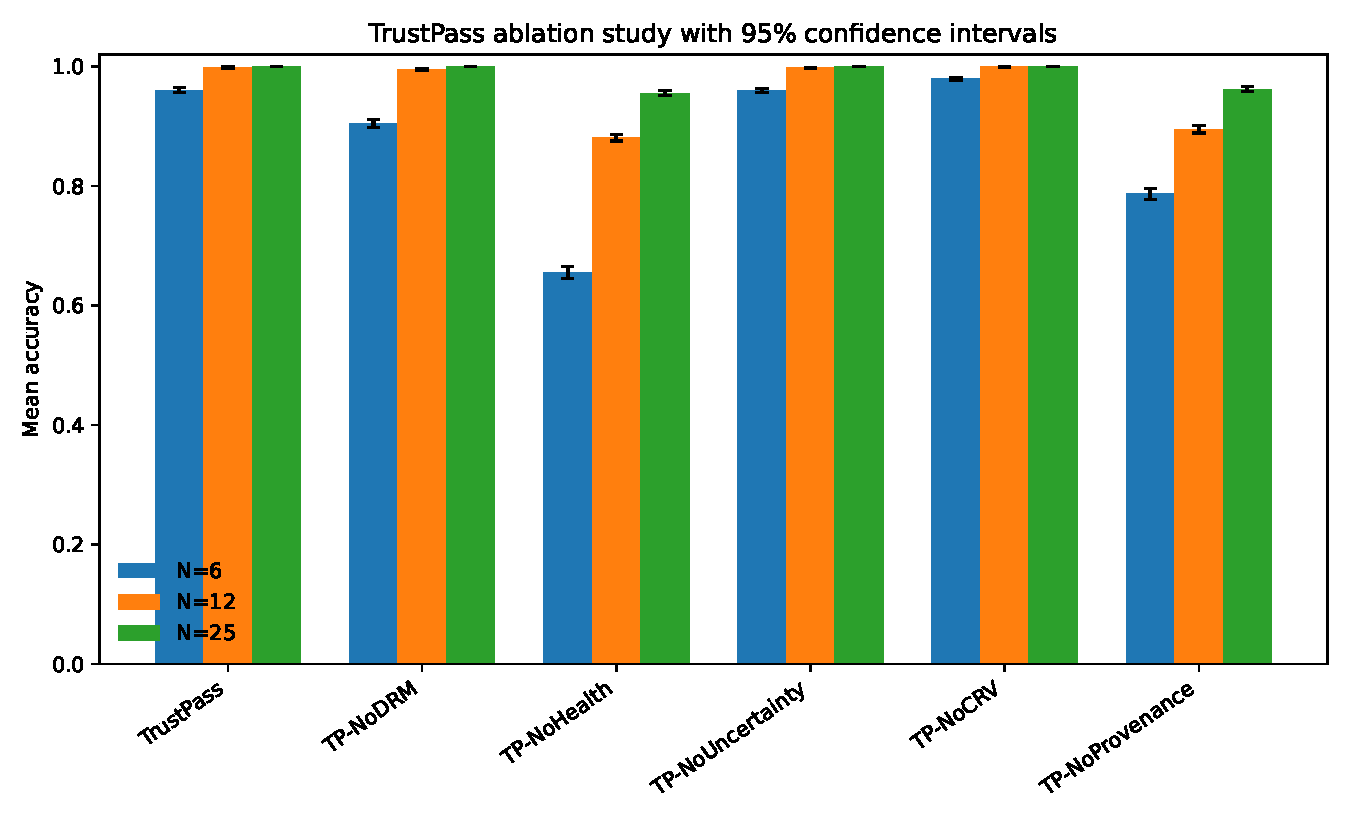
\includegraphics[width=0.98\linewidth]{results_extended_v2/ablation_accuracy.pdf}
  \caption{Corrected TrustPass ablation results with 95\% confidence intervals.}
  \label{fig:ablation}
\end{figure}

\subsection{Attack-Intensity Sweep}

Table~\ref{tab:attack-sweep} reports the attack sweep at $N=12$.

\begin{table}[t]
\centering
\caption{Accuracy under increasing compromised-agent fractions at $N=12$.}
\label{tab:attack-sweep}
\scriptsize
\begin{tabular}{ccccc}
\toprule
Compromised & TrustPass & DS-Trust & EBT & Majority \\
\midrule
0.10 & 0.999 & 0.998 & 0.998 & 0.998 \\
0.20 & 0.998 & 0.997 & 0.997 & 0.993 \\
0.30 & 0.993 & 0.978 & 0.982 & 0.954 \\
0.40 & 0.990 & 0.952 & 0.957 & 0.898 \\
0.50 & 0.975 & 0.925 & 0.926 & 0.800 \\
0.60 & 0.965 & 0.869 & 0.862 & 0.675 \\
0.70 & 0.922 & 0.781 & 0.757 & 0.544 \\
\bottomrule
\end{tabular}
\end{table}

TrustPass accuracy decreases as the compromised-agent fraction increases but remains above the baselines throughout the tested sweep. At 70\% compromised agents, TrustPass reaches 0.922, compared with 0.781 for DS-Trust, 0.757 for EBT, and 0.544 for Majority.

These results should be interpreted as resilience within the simulator's threat model, not as a general guarantee against arbitrary collusion or compromise.

\begin{figure}[t]
  \centering
  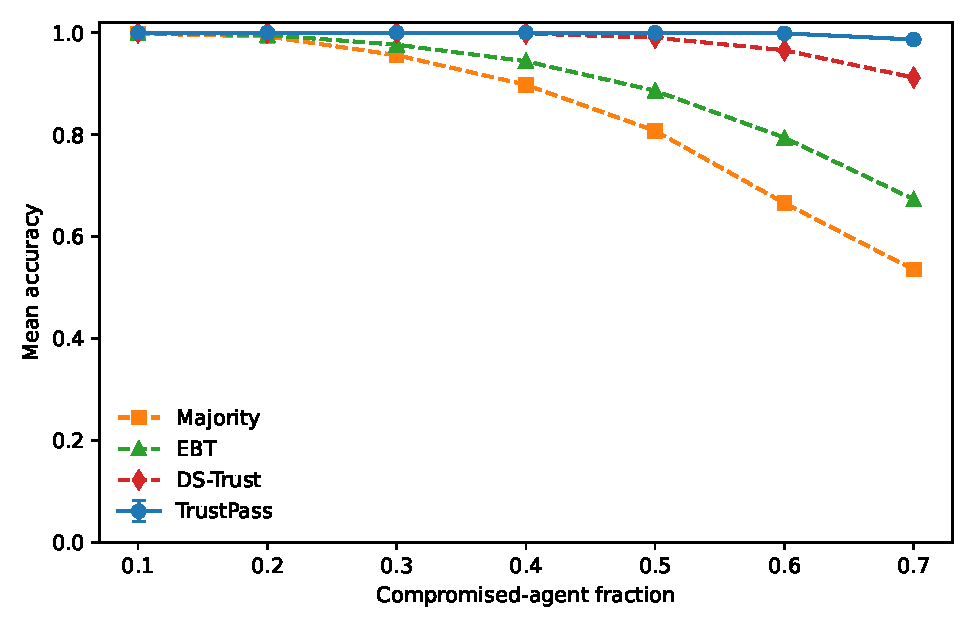
\includegraphics[width=0.98\linewidth]{results_extended_v2/attack_sweep.pdf}
  \caption{Accuracy as the fraction of compromised agents increases. Error bars show 95\% confidence intervals for TrustPass.}
  \label{fig:attack-sweep}
\end{figure}

\subsection{Packet-Loss Sweep}

Table~\ref{tab:packet-loss} reports performance at increasing packet-loss rates.

\begin{table}[t]
\centering
\caption{Accuracy under packet loss at $N=12$, with 55\% compromised agents and 12\% relay compromise.}
\label{tab:packet-loss}
\scriptsize
\begin{tabular}{cccc}
\toprule
Packet loss & TrustPass & EBT & Majority \\
\midrule
0.00 & 0.963 & 0.858 & 0.674 \\
0.10 & 0.945 & 0.839 & 0.670 \\
0.20 & 0.930 & 0.820 & 0.655 \\
0.30 & 0.914 & 0.800 & 0.623 \\
0.40 & 0.890 & 0.778 & 0.586 \\
0.50 & 0.862 & 0.756 & 0.563 \\
\bottomrule
\end{tabular}
\end{table}

At 50\% packet loss, TrustPass accuracy decreases to 0.862 but remains above EBT at 0.756 and Majority at 0.563. This indicates graceful degradation under the tested missing-evidence model. The result does not establish performance under real DTN scheduling, bandwidth constraints, propagation delay, or correlated packet loss.

\begin{figure}[t]
  \centering
  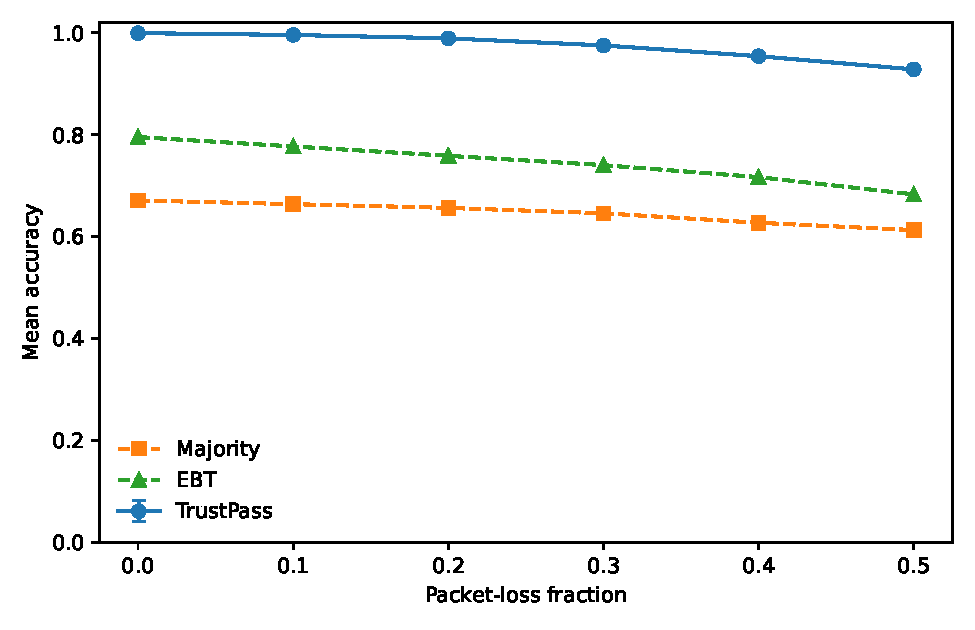
\includegraphics[width=0.98\linewidth]{results_extended_v2/packet_loss_sweep.pdf}
  \caption{Accuracy under packet loss. Missing packets are excluded from aggregation rather than treated as negative claims.}
  \label{fig:packet-loss}
\end{figure}

\section{Discussion}
\label{sec:discussion}

The revised evaluation changes the interpretation of TRUSTPASS in an important way. The results do not show that every architectural component improves accuracy in every regime. Instead, sensor-health and provenance/integrity weighting provide the strongest measured contributions. Dynamic reputation is most useful when the constellation is small. Uncertainty weighting has little measurable effect under the current calibration. The population-agreement CRV heuristic slightly reduces performance at small constellation sizes.

The CRV result is informative. A verifier that estimates consensus from the received population can be misled when compromised agents form the majority or when relay manipulation changes the apparent distribution. This motivates future CRV designs based on independent sensor modalities, provenance diversity, trusted anchors, temporal consistency, and explicit common-mode-failure detection.

The provenance result should also be interpreted carefully. The simulator uses synthetic provenance-quality and integrity attributes rather than real signed PROV graphs. The result therefore supports the value of provenance/integrity weighting as a modeled mechanism, not the effectiveness of a particular provenance standard or cryptographic protocol.

The attack sweep shows that TrustPass remains more accurate than the selected baselines as the compromised-agent fraction increases from 10\% to 70\%. This is a result within the implemented threat model. It should not be generalized to arbitrary attackers that compromise signing keys, corrupt all independent sensors, or coordinate perfectly across the entire network.

The packet-loss sweep shows graceful degradation under independently missing packets. Real deep-space operation also requires modeling delay distributions, contact windows, bundle expiration, bandwidth scheduling, correlated outages, and delayed feedback. These are important directions for future work.

\section{Threats to Validity}
\label{sec:validity}

\textbf{Synthetic environment.}
The simulator uses binary phenomena, Gaussian sensor noise, synthetic provenance quality, synthetic integrity outcomes, and simplified adversarial behavior. It does not reproduce real spacecraft telemetry or planetary science workflows.

\textbf{Parameter selection.}
The original adversarial regime was selected to avoid majority-vote saturation. The revised sweeps broaden the tested range, but they do not constitute a complete factorial sensitivity analysis.

\textbf{Ground-truth feedback.}
Ground truth is available to the simulator for offline scoring and reputation feedback. An operational spacecraft would receive delayed validation rather than immediate ground truth.

\textbf{CRV model.}
The current CRV implementation uses a population-agreement heuristic. It can reinforce a false consensus when compromised agents dominate the received reports. More robust independence and common-mode-failure models are required.

\textbf{Provenance model.}
The experiment uses synthetic provenance-quality and integrity attributes. It does not implement full PROV-DM, PROV-AGENT, secure hardware roots, or cryptographic key-management protocols.

\textbf{Statistical scope.}
Each configuration uses 80 trials and reports normal-approximation 95\% confidence intervals. The experiment does not provide a formal proof of security or statistical guarantees for all missions.

\section{Conclusion}
\label{sec:conclusion}

This paper framed cybersecurity assurance of AI-generated scientific claims in autonomous deep-space multi-agent systems as a distinct research problem. The proposed TRUSTPASS architecture combines machine-verifiable evidence packages, sensor-health assessment, provenance and integrity metadata, cross-relay verification, and dynamic reputation.

The revised evaluation adds component ablations, attack-intensity sweeps, packet-loss experiments, and confidence intervals. Under the tested synthetic threat model, sensor-health and provenance/integrity weighting provide the strongest contributions, while dynamic reputation is most useful for smaller constellations. The current CRV heuristic does not improve accuracy in every configuration and can slightly reinforce misleading consensus. These findings identify both the value and the limitations of integrating evidence quality and trust mechanisms.

The results are a controlled proof of concept rather than a mission-ready validation. Future work should implement real provenance graphs, cryptographic attestation, independent sensor modalities, realistic DTN contact schedules, delayed-feedback reputation, stronger collusion models, and high-fidelity autonomous-science workflows.

\section*{Acknowledgment}

The author thanks the open-source community for tools and datasets that supported this work. This research was conducted without specific grant support.

\section*{Declarations}

\subsection*{Competing Interests}

The author declares that there are no financial or non-financial competing interests related to this work.

\subsection*{Funding}

No funding was received for conducting this study or preparing this manuscript.

\subsection*{Data Availability}

The simulation scripts, configuration, random seeds, raw trial records, generated summary CSV files, and figures are available at:

\url{https://github.com/netclouts/deep-space-trustpass}

The study uses synthetic observations and contains no restricted spacecraft telemetry or personally identifiable research data.

\bibliographystyle{IEEEtran}
\bibliography{references}

\end{document}
